\section{Fields, Metrics, and Space-Time Symmetry}
\subsection{Review - Coordinates, Transformations, Scalar Fields}
Last time, we were considering a coordinate system for our spacetime (which has requirements such as smoothness that we take as a given); we have a four-vector $x^\mu$ which represents a point in the spacetime. We then considered a different coordinate system $\tilde{x}^\mu$ and a change-of-coordinates transformation $x^\mu \to \tilde{x}^\mu(x)$ (four smooth functions in four variables). This function should be invertible, with $\tilde{x}^\mu \to x^\mu(\tilde{x})$ the inverse.

We can then discuss things that live in our spacetime, such as the scalar field. The term scalar says something about this; namely it tells us how we should translate values of the field under different coordinate transformations. We have some scalar field $\varphi(x)$, and in some different set of coordinates we may have $\tilde{\varphi}(\tilde{x})$ but at the same point the data should match, so:
\begin{equation}
    \varphi(x) = \tilde{\varphi}(\tilde{x})
\end{equation}

\subsection{Vector Fields}
This is a straightforward generalization of a vector field; at each point in space we associate a vector with magnitude and direction. If temperature was an example of a scalar field, then wind would be a good example of a vector field; the wind has some magnitude and direction at each point in space. But now something to consider; when we transform between coordinates, we not only have to translate magnitudes, but also the direction of the wind. We say a (contravariant) vector field should transform like a differential:
\begin{equation}
    dx^\mu = \dpd{x^\mu}{\tilde{x}^\mu}d\tilde{x}^\nu
\end{equation}
so:
\begin{equation}
    A^\mu(x) = \dpd{x^\mu}{\tilde{x}^\nu}\tilde{A}^\nu(\tilde{x})
\end{equation}
note the up and down indices here are quite important. $x$ always has an up index. The index on the derivative is a bit interesting. We consider a transformation of the derivative:
\begin{equation}
    \dpd{}{x^\nu} = \dpd{\tilde{x}^\nu}{x^\mu}\dpd{}{\tilde{x}^\nu}
\end{equation}
and we see that this is upside-down compared to the vector field transformation; so something different is happening here. We could find a vector field that transforms under this ``upside-down'' rule, and we would distinguish this by putting a down index on it (this would be a covariant) vector field:
\begin{equation}
    A_\mu(x) = \dpd{\tilde{x}^\nu}{x^\mu}\tilde{A}_\nu(\tilde{x})
\end{equation}
Note: we remind the reader that we work with Einstein summation convention, and so when we have two indices paired they are summed over. Since the partial derivative transforms covariantly, it is natural to think of it as an object as a down index:
\begin{equation}
    \p_\mu = \dpd{}{x^\mu}, \quad \tilde{\p}_\mu = \dpd{}{\tilde{x}^\mu}
\end{equation}

\subsection{Tensor Fields}
Tensor fields are a generalization of vector fields; they are things with more than one index. One example is the inertia tensor with two indices takes the form of a 3x3 matrix in 3-dimensional space. The relativistic description of an EM field is another. We can lift our transformations of vectors into tensors in the most obvious way:
\begin{equation}
    \mathbb{T}^{\mu_1 \ldots \mu_m}\nu_{1 \ldots n}(x) = \dpd{x^{\mu_1}}{\tilde{x}^{\rho_1}}\ldots \dpd{x^{\mu_m}}{\tilde{x}^{\rho_m}} \dpd{\tilde{x}^{\sigma_1}}{x^{\nu_1}}\ldots \dpd{\tilde{x}^{\sigma_n}}{x^{\nu_n}}\tilde{\mathbb{T}}^{\rho_1 \ldots \rho_m}_{\sigma_1 \ldots \sigma_n}(\tilde{x})
\end{equation}

\subsection{Proper Time and Spacetime Metrics}
At this point, we know nothing about the spacetime beyond the fact that I know I can index it and measure things. We need more than that; we will need to embed objects into this spacetime somehow. We will need some rules for doing so, and rules thar we can all agree on.

Let's take a pet snail\footnote{Let's assume that snails exist...} and put him at $x^\mu$ in our spacetime. Now let's say he moves to $x^\mu + dx^\mu$. We then record the time that elapses on the wristwatch. This we would call the proper time. 

\begin{figure}[htbp]
    \centering
    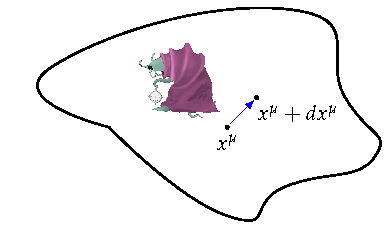
\includegraphics[]{Images/fig-propertime.pdf}

    \caption{We take our pet snail (actually pictured is a slug, but close enough) and put him at coordinate $x^\mu$ in our spacetime. We then define the proper time as the time that elapses on his watch when he moves from $x^\mu$ to $x^\mu + dx^\mu$.}
    \label{<label>}
\end{figure}

This should vary linearly with how far he travells. We should also have a perscription for the path taken to be somehow ``sensible''; say $x^\mu + tdx^\mu$ for $0 \leq t \leq 1$. We want some way of figuring out what this proper time is. If it's linear in $x^\mu$, but this has an index and proper time is just a number. So it would be useful to square the propert time; this would be bi-linear in $x^\mu$, perhaps with an expression:
\begin{equation}
    d\tau^2 = dx^\mu g_{\mu\nu}(x)dx^\nu
\end{equation}
this defines a matrix $g_{\mu\nu}$ of some kind. It turns out to be a fairly special one; why? If we both watch the snail and record the proper time in the same way, we should agree on that proper time for every possible path he should take. We can therefore map out this matrix. Even if we restrict ourselves to timelike paths, there is enough to map out this tensor. The physics tells us that the times must agree, and so:
\begin{equation}\label{eq-dtau2WC}
    d\tau^2 = dx^\mu g_{\mu\nu}(x)dx^\nu = d\tilde{x}^\mu \tilde{g}_{\mu\nu}(\tilde{x})d\tilde{x}^\nu
\end{equation}
This tells us that $g$ transforms as a tensor field! And so:
\begin{equation}
    g_{\mu\nu}(x) = \dpd{\tilde{x}^\rho}{x^\mu}\dpd{\tilde{x}^\sigma}{x^\nu}\tilde{g}_{\rho\sigma}(\tilde{x}).
\end{equation}
We give this tensor field a name of being a \emph{metric}, or \emph{metric tensor}. This encodes a lot of information about our spacetime, as it in a sense measures distances. We will not go into the direction of curvature and general relativity here, but this is certainly a fascinating direction. 

\subsection{Minkowski Spacetime}
We are only example in a specific example of spacetime - Minkowski spacetime. We define it as a spacetime where there exists a coordinate system such that:
\begin{equation}
    g_{\mu\nu}(x) = \m{-1& 0 & 0 & 0 \\ 0 & 1 & 0 & 0 \\ 0 & 0 & 1 & 0 \\ 0 & 0 & 0 & 1}
\end{equation}
the poor snail notices that there are limits on his motion coming from the minus sign; he cannot for example go backwards in time. Note we have to correct the formula in Eq. \eqref{eq-dtau2WC} we had for $d\tau^2$ due to this minus sign:
\begin{equation}
    d\tau^2 = -dx^\mu g_{\mu\nu}(x)dx^\nu = -d\tilde{x}^\mu \tilde{g}_{\mu\nu}(\tilde{x})d\tilde{x}^\nu
\end{equation}
Note that this is known as the east-coast convention; one could alternatively take:
\begin{equation}
    g_{\mu\nu}(x) = \m{1& 0 & 0 & 0 \\ 0 & -1 & 0 & 0 \\ 0 & 0 & -1 & 0 \\ 0 & 0 & 0 & -1}
\end{equation}
and this would be the west-coast convention. Despite our location at UBC, we adopt the east-coast convention.

Some background; the WC convention was developed by high-energy physicists, while the EC convention was developed by relativists. The former has the benefit of energies being positive, the latter has the benefit of distances being positive. Both are correct and often one takes the convention most convenient for the setting (depending on whether you discuss particle energies, or geometry).

\subsection{Infinitesimal Coordinate Transformations}
We consider infinitesimal coordinate transformations:
\begin{equation}
    \tilde{x}^\mu = x^\mu + f^\mu(x)
\end{equation}
We can think of $f^\mu$ as small but otherwise arbitrary. It also looks like a vector field, but is not quite one (it coordinate transforms in a funny way). Scalar fields transform under infinitesimal transformations as:
\begin{equation}
    \varphi(x) = \tilde{\varphi}(\tilde{x}) = \varphi(x) + \delta \varphi(x) + f^\mu(x)\p_\mu\varphi(x)
\end{equation}
where we have Taylor expanded in $f$ for the last term. As usual we consider only up to linear order. Cancelling terms, we obtain:
\begin{equation}
    \delta \phi(x) = -f^\mu(x)\p_\mu\phi(x)
\end{equation}
We can then abstract this to various other fields. One example is the contravariant vector field:
\begin{equation}
    A^\mu(x) = \dpd{x^\mu}{\tilde{x}^\nu}\tilde{A}^{\nu}(\tilde{x})
\end{equation}
Note the beauty of infinitesimal transformations in that they are very easy to invert:
\begin{equation}
    x^\mu = \tilde{x}^\mu - f^\mu(\tilde{x})
\end{equation}
and so
\begin{equation}
    \dpd{x^\mu}{\tilde{x}^\nu} = \delta^\mu_\nu - \p_\nu f^\mu
\end{equation}
therefore:
\begin{equation}
    A^\mu(x) = A^\mu(x) - \p_\nu f^{\mu}(x)A^\nu(x) + \delta A^\mu(x) + f^\nu(x)\p_\nu A^\mu(x)
\end{equation}
From here the zeroth order bit cancells out, and so:
\begin{equation}
    \delta A^\mu(x) = -f^\nu\p_\nu A^\mu(x) + \p_\nu f^\mu(x)A^\nu(x)
\end{equation}
where the first term comes from the transformation of the coordinate and the second term comes from the transformation of the frame. The scalar field has the first part (and in fact every field will have it)! The extra terms are the derivatives of the transformation function with the indices matched up. Doing the same for covariant fields:
\begin{equation}
    \delta A_\mu(x) = -f^\nu(x)\p_\nu A_\mu(x) - \p_\mu f^\nu(x) A_\nu(x)
\end{equation}
And as a particular example, the metric transforms as:
\begin{equation}
    \delta g_{\mu\nu}(x)=  - f^\lambda(x)\p_\lambda g_{\mu\nu}(x) - \p_\mu f^\lambda(x) g_{\lambda \nu}(x) - \p_\nu f^\lambda(x) g_{\mu\lambda}(x)
\end{equation}

\subsection{The definition of space-time symmetry}
Having discussed metrics, what else can one say about a space? One thing that would be interesting is symmetry. Maybe we can define symmetry of spacetime as follows; symmetry is a change of coordinates such that the rules for calculating proper time remain exactly the same. We need the metric to calculate the proper time; so if we calculate the same proper time under a coordinate transformation, the metric better be left identical. Putting this together, we can say that \emph{A symmetry of space-time is a coordinate transformation such that $\delta g_{\mu\nu}(x) = 0$}. So to discover symmetries, we can dream up a large class of $f$s, and see for what class we have $\delta g_{\mu\nu}(x) = 0$. This wouldn't be a useful definition of symmetry was plentiful, and in general it is quite rare to find them. Precisely, the maximum number of spacetime symmetries turns out to be $d(d+1)/2$\footnote{The number of independent components of a $d\times d$ symmetric tensor - though typically there are less, there are only 3 maximally symmetric spaces, namely Minkowski, and the spaces of constant positive or constant negative curvature. For 2D surfaces, this means the only maximally symmetric surfaces are the plane, sphere, and the one that looks locally like a Pringle (I missed the formal name that Gordon said here). In 4D we have Minkowski, DeSitter and Anti DeSitter space.}. This is obtained by counting the solutions to the differential equation obtained by setting $\delta g_{\mu\nu}(x) = 0$. An equivalent definition of symmetry is therefore: \emph{$\hat{f}^\mu(x)$ is a symmetry if:
\begin{equation}
    \hat{f}^\lambda(x)\p_\lambda g_{\mu\nu}(x) + \p_\mu \hat{f}^\lambda(x) g_{\lambda \nu}(x) + \p_\nu \hat{f}^\lambda(x) g_{\mu\lambda}(x)
\end{equation}
i.e. $\hat{f}^\mu(x)$ the Killing vector satisfies the Killing equation.} One might wonder if the form of the equation changes in different coordinate systems; this turns out to not be the case (and would require some differential geometry knowledge). This gives us a systematic way to discuss symmetries; something we will continue with next class.